\documentclass[10pt, a4paper]{exam}
\printanswers			    % Comment this line to hide the answers 
\usepackage[utf8]{inputenc}
\usepackage[T1]{fontenc}
\usepackage[ngerman]{babel}
\usepackage{amsmath,amsthm,amsfonts,amssymb}
\usepackage[many]{tcolorbox}
\usepackage{pgfplots}
\pgfplotsset{compat=1.17}

\pdfinfo{
    /Title (Grundlagen und diskrete Strukturen - Übung)
    /Creator (TeX)
    /Producer (pdfTeX 1.40.0)
    /Author ()
    /Subject ()
}
\title{Grundlagen und diskrete Strukturen - Übung}
\author{}
\date{}

% Don't print section numbers
\setcounter{secnumdepth}{0}
\qformat{\textbf{Aufgabe \thequestion}\dotfill \thepoints}

\newtcolorbox{myboxii}[1][]{
  breakable,
  freelance,
  title=#1,
  colback=white,
  colbacktitle=white,
  coltitle=black,
  fonttitle=\bfseries,
  bottomrule=0pt,
  boxrule=0pt,
  colframe=white,
  overlay unbroken and first={
  \draw[red!75!black,line width=3pt]
    ([xshift=5pt]frame.north west) -- 
    (frame.north west) -- 
    (frame.south west);
  \draw[red!75!black,line width=3pt]
    ([xshift=-5pt]frame.north east) -- 
    (frame.north east) -- 
    (frame.south east);
  },
  overlay unbroken app={
  \draw[red!75!black,line width=3pt,line cap=rect]
    (frame.south west) -- 
    ([xshift=5pt]frame.south west);
  \draw[red!75!black,line width=3pt,line cap=rect]
    (frame.south east) -- 
    ([xshift=-5pt]frame.south east);
  },
  overlay middle and last={
  \draw[red!75!black,line width=3pt]
    (frame.north west) -- 
    (frame.south west);
  \draw[red!75!black,line width=3pt]
    (frame.north east) -- 
    (frame.south east);
  },
  overlay last app={
  \draw[red!75!black,line width=3pt,line cap=rect]
    (frame.south west) --
    ([xshift=5pt]frame.south west);
  \draw[red!75!black,line width=3pt,line cap=rect]
    (frame.south east) --
    ([xshift=-5pt]frame.south east);
  },
}

\begin{document}

\begin{myboxii}[Disclaimer]
    Die Übungen die hier gezeigt werden stammen aus der Vorlesung \textit{Grundlagen und diskrete Strukturen}! Für die Richtigkeit der Lösungen wird keine Gewähr gegeben.
\end{myboxii}

%##########################################
\begin{questions}
    \question Welche der folgenden Sätze sind logische Aussagen? Geben Sie, falls möglich, den Wahrheitswert mit Begründung an.
    \begin{parts}
        \part  Es gibt unendlich viele Primzahlen.
        \begin{solution}
            Ist eine Aussage, es gibt entweder unendlich viele Primzahlen oder nicht. Nach Euklid ist diese Aussage wahr: "Satz von Euklid"
        \end{solution}
        \part Hat die Gleichung $x^3-x = 0$ zwei reelle Lösungen?
        \begin{solution}
            Ist eine Aussage, entweder stimmt die Aussage und die Gleichung hat zwei reelle Lösungen oder es gibt keine oder mehr reelle Lösungen. Die Gleichung hat tatsächlich drei Lösungen $(-1,0,-1)$, damit ist die Aussage falsch.
        \end{solution}
        \part Dieser Satz besteht aus sechs Wörtern.
        \begin{solution}
            Ist eine Aussage und ist wahr.
        \end{solution}
        \part Dieser Satz ist falsch.
        \begin{solution}
            Ist eine keine Aussage. Wäre er wahr, so wäre er nach eigener Aussage falsch. Ist ein "Antinomien".
        \end{solution}
        \part Ein Satz, der das Wort Steuersenkung enthält ist falsch.
        \begin{solution}
            Ist eine Aussage die einem Wahrheitswert zugewiesen werden kann. Der Wahrheitswert ist falsch, da mindestens ein Satz existiert der das Wort Steuersenkung enthält und wahr ist.
        \end{solution}
        \part Es gibt einen Gott.
        \begin{solution}
            Ist keine Aussage. Dem Satz kann kein Wahrheitswert oder eindeutige Bedeutung zugewiesen werden.
        \end{solution}
        \part Wenn Rot gleich Grün ist, dann ist Schwarz gleich Gelb.
        \begin{solution}
            Ist keine Aussage. Werten Rot, Grün usw. kann man keinen eindeutigen Eigenwert zuweisen (Additiv, Substraktiv, ...). Damit kann auch kein Wahrheitswert zugewiesen werden.
        \end{solution}
    \end{parts}

    \question Bestimmen Sie den Wahrheitswerteverlauf der aussagenlogischen Formel $((p \leftrightarrow q) \wedge q) \rightarrow p$.
    \begin{solution}

        \begin{tabular}{c c c c c}
            $p$ & $q$ & $x=(p\leftrightarrow q)$ & $y=(x\wedge q)$ & $y\rightarrow p$ \\\hline
            0   & 0   & 1                        & 0               & 1                \\
            0   & 1   & 0                        & 0               & 1                \\
            1   & 0   & 0                        & 0               & 0                \\
            1   & 1   & 1                        & 1               & 1                \\
        \end{tabular}
    \end{solution}

    \question Untersuchen Sie mit Hilfe aussagenlogischer Formeln, ob sich die folgende Argumentation als Beweis dafür eignet , dass 7 eine Primzahl ist. Aus der Aussage ,,Wenn 7 kleiner ist als 4, dann ist 7 keine Primzahl.'' und der Aussage ,,7 ist nicht kleiner als 4'' folgt die Aussage ,,7 ist eine Primzahl.''
    \begin{solution}
        \begin{itemize}
            \item $a: (7<4)\rightarrow 7\not\in Prim$
            \item $b: (7\not<4)\rightarrow 7\in Prim$
            \item $c: 7>4 \rightarrow wahr$
            \item $c\rightarrow \bar{a} \cup b \rightarrow \lnot(7\not\in Prim) \cup 7\in Prim \Rightarrow 7\in Prim$
        \end{itemize}
    \end{solution}

    \question Welche der folgenden aussagenlogischen Formeln sind Tautologien bzw. Kontradiktionen?
    \begin{parts}
        \part $(p \wedge (p \rightarrow q)) \rightarrow q$
        \begin{solution}

            \begin{tabular}{ccccc}
                $p$ & $q$ & $x:p\rightarrow q$ & $y:p\wedge x$ & $y\rightarrow q$ \\\hline
                0   & 0   & 1                  & 0             & 1                \\
                0   & 1   & 1                  & 0             & 1                \\
                1   & 0   & 0                  & 0             & 1                \\
                1   & 1   & 1                  & 1             & 1                \\
            \end{tabular}

            ist Tautologie
        \end{solution}
        \part $(\lnot p \vee (\lnot p \wedge q)) \leftrightarrow p$
        \begin{solution}

            \begin{tabular}{ccccc}
                $p$ & $q$ & $x:\lnot p\wedge q$ & $y:\lnot p\vee x$ & $y\leftrightarrow q$ \\\hline
                0   & 0   & 0                   & 1                 & 1                    \\
                0   & 1   & 1                   & 1                 & 1                    \\
                1   & 0   & 0                   & 0                 & 1                    \\
                1   & 1   & 0                   & 0                 & 1                    \\
            \end{tabular}

            alternativ umwandeln: $((\lnot p\vee\lnot p)\wedge(\lnot p\vee q))\leftrightarrow p\Rightarrow (\lnot p\vee q)\leftrightarrow p$

            ist Tautologie
        \end{solution}
        \part $(p \leftrightarrow q) \leftrightarrow (\lnot p \leftrightarrow \lnot q)$
        \begin{solution}

            \begin{tabular}{ccccc}
                $p$ & $q$ & $x:p\leftrightarrow q$ & $y:\lnot p\leftrightarrow \lnot q$ & $x\leftrightarrow y$ \\\hline
                0   & 0   & 1                      & 1                                  & 1                    \\
                0   & 1   & 0                      & 0                                  & 1                    \\
                1   & 0   & 0                      & 0                                  & 1                    \\
                1   & 1   & 1                      & 1                                  & 1                    \\
            \end{tabular}

            ist Tautologie
        \end{solution}
    \end{parts}

    \question Beweisen Sie die folgenden logischen Äquivalenzen.
    \begin{parts}
        \part $p\equiv (p \wedge (p \vee q))$
        \begin{solution}

            \begin{tabular}{cccc}
                $p$ & $q$ & $p\vee q$ & $p\wedge(p\vee q)$ \\\hline
                0   & 0   & 0         & 0                  \\
                0   & 1   & 1         & 0                  \\
                1   & 0   & 1         & 1                  \\
                1   & 1   & 1         & 1                  \\
            \end{tabular}
        \end{solution}
        \part $(p \wedge (q \wedge r)) \equiv ((p \wedge q) \wedge r)$
        \begin{solution}

            \begin{tabular}{cccccccc}
                $p$ & $q$ & $r$ & $(q \wedge r)$ & $x: (p \wedge (q \wedge r)$ & $p \wedge q$ & $y: (p \wedge q) \wedge r$ & $x\equiv y$ \\\hline
                0   & 0   & 0   & 0              & 0                           & 0            & 0                          & 1           \\
                0   & 0   & 1   & 0              & 0                           & 0            & 0                          & 1           \\
                0   & 1   & 0   & 0              & 0                           & 0            & 0                          & 1           \\
                0   & 1   & 1   & 0              & 0                           & 0            & 0                          & 1           \\
                1   & 0   & 0   & 0              & 0                           & 0            & 0                          & 1           \\
                1   & 0   & 1   & 1              & 0                           & 0            & 0                          & 1           \\
                1   & 1   & 0   & 0              & 0                           & 1            & 0                          & 1           \\
                1   & 1   & 1   & 1              & 1                           & 1            & 1                          & 1           \\
            \end{tabular}
        \end{solution}
        \part $(p \wedge (q \vee r)) \equiv ((p \wedge q) \vee (p \wedge r))$
        \begin{solution}

            \begin{tabular}{ccccccccc}
                $p$ & $q$ & $r$ & $q\vee r$ & $x:p\wedge(q\vee r)$ & $a:p\wedge q$ & $b:p\wedge r$ & $y:a\vee b$ & $x\equiv y$ \\\hline
                0   & 0   & 0   & 0         & 0                    & 0             & 0             & 0           & 1           \\
                0   & 0   & 1   & 1         & 0                    & 0             & 0             & 0           & 1           \\
                0   & 1   & 0   & 1         & 0                    & 0             & 0             & 0           & 1           \\
                0   & 1   & 1   & 1         & 0                    & 0             & 0             & 0           & 1           \\
                1   & 0   & 0   & 0         & 0                    & 0             & 0             & 0           & 1           \\
                1   & 0   & 1   & 1         & 1                    & 0             & 1             & 1           & 1           \\
                1   & 1   & 0   & 1         & 1                    & 1             & 0             & 1           & 1           \\
                1   & 1   & 1   & 1         & 1                    & 1             & 1             & 1           & 1           \\
            \end{tabular}
        \end{solution}
        \part $(\lnot(p \wedge q)) \equiv ((\lnot p) \vee (\lnot q))$
        \begin{solution}

            \begin{tabular}{ccccc}
                $p$ & $q$ & $x:\lnot(p\wedge q)$ & $y:\lnot p \vee \lnot q$ & $x\equiv y$ \\\hline
                0   & 0   & 1                    & 1                        & 1           \\
                0   & 1   & 1                    & 1                        & 1           \\
                1   & 0   & 1                    & 1                        & 1           \\
                1   & 1   & 0                    & 0                        & 1           \\
            \end{tabular}
        \end{solution}
    \end{parts}

    \question Beweisen Sie:
    \begin{parts}
        \part Jede Aussagenlogische Formel ist äquivalent zu einer aussagenlogischen Formel, in der die konstanten Wahrheitswerte w und f nicht vorkommen.
        \begin{solution}

        \end{solution}
        \part Jede Aussagenlogische Formel ist äquivalent zu einer aussagenlogischen Formel, in der weder Implikation noch Äquivalenz vorkommt.
        \begin{solution}
            $p\wedge q \vee r \not\equiv p\vee q\wedge r $

            $\Rightarrow$ nicht jede
        \end{solution}
    \end{parts}

    \question Auf einer Insel leben nur Ritter und Schurken. Die Ritter sagen immer die Wahrheit, und die Schurken lügen immer. Wir treffen auf der Insel drei Personen A, B und C. A sagt: ,,Jeder von uns dreien ist ein Schurke,'' B sagt: ,,Genau einer von uns dreien ist ein Ritter.'' Der Vollständigkeit und guten Ordnung halber sei erwähnt, dass C schweigt. Was sind A, B und C?
    \begin{solution}
        Ist Aussage A richtig, dann sind alle Schurken und lügen. Aber wenn alle Schurken sind, wäre dieser Satz gelogen und ist damit falsch. Daraus folgt, dass mindestens ein Ritter existieren muss.
        Sei Aussage B richtig, dann ist genau einer von dreien ein Ritter. Wenn B richtig ist, sagt B die Wahrheit und ist damit ein Ritter, die anderen beiden Schurken.
        Sei Aussage B falsch, dann müssen es zwei Ritter sein. Es kann nicht nur Schurken geben, da sonst A wahr wäre. Dann wären B und C Ritter, A ist bereits Schurke. Aber wenn B ein Ritter sein soll, wäre seine Aussage wahr und widerspricht den zwei Rittern.
        Deshalb ist B wahr, B ein Ritter und C ein Schurke.
    \end{solution}

    \question Geben Sie für die Aussageform $p(x) = $,,x ist nicht durch zwei teilbar'' Universen $U_1,U_2,U_3$ und $U_4$ mit unendlich vielen Elementen so an, dass
    \begin{parts}
        \part ,,$\forall x \in U_1 : p(x)$,, wahr ist,
        \begin{solution}
            $U_1 = \{z | \text{z ist ungerade}\}$
        \end{solution}
        \part ,,$\forall x \in U_2 : p(x)$,, falsch ist,
        \begin{solution}
            $U_2 = \{z | \text{ z ist gerade}\}$
        \end{solution}
        \part ,,$\exists x \in U_3 : p(x)$,, wahr ist,
        \begin{solution}
            $U_3 = \mathbb{R}$
        \end{solution}
        \part ,,$\exists x \in U_4 : p(x)$,, falsch ist.
        \begin{solution}
            $U_4 = \mathbb{R}$
        \end{solution}
    \end{parts}

    \question Stellen Sie den folgenden mathematischen Sachverhalt als Aussageform dar:
    ,,Das arithmetische Mittel verschiedener positiver reeller Zahlen ist größer als deren geometrisches Mittel.''
    \begin{solution}
        $ x_{arit} > x_{geom} \Rightarrow \frac{1}{n}\sum_{i=1}^n x_i > \sqrt[n]{\prod_{i=1}^n x_i}$

    \end{solution}

    \question Bilden Sie die Negation folgender Aussagen:
    \begin{parts}
        \part Für jedes Töpfchen gibt es ein Deckelchen.
        \begin{solution}
            Es gibt mindestens einen Topf ohne Deckel.
        \end{solution}
        \part Immer, wenn ich nach Ilmenau komme, regnet es oder die Schranken sind unten.
        \begin{solution}
            Es gibt mindestens ein mal nach dem ich in Ilmenau komme, dass es nicht rechnet und nicht die Schranken unten sind.
        \end{solution}
        \part Für jeden Studierenden gibt es mindestens eine interessante Vorlesung.
        \begin{solution}
            Es gibt mindestens einen Studenten für den es es keine interessante Vorlesung gibt.
        \end{solution}
        \part Everybody loves somebody sometimes.
        \begin{solution}
            Somebody loves nobody anytime.
        \end{solution}
        \part Kleine Kinder und Betrunkene sagen immer die Wahrheit.
        \begin{solution}
            Kleine Kinder und Betrunkene sagen nicht immer die Wahrheit.
        \end{solution}
        \part $\forall \epsilon > 0 \exists N \in\mathbb{N}\forall n > N: |a_n - g| < \epsilon \quad\quad (lim_{n\rightarrow\infty} a_n = g)$
        \begin{solution}
        \end{solution}
        \part $\forall S\in\mathbb{R} \exists N\in\mathbb{N}\forall n > N: a_n > S \quad\quad (lim_{n\rightarrow\infty} a_n = +\infty)$
        \begin{solution}
        \end{solution}
    \end{parts}

    \question Welche der folgenden Äquivalenzen gelten für jedes Universum und beliebige Prädikate P, Q?
    \begin{parts}
        \part $\forall x(P (x) \vee Q(x)) \equiv  (\forall xP (x)) \vee (\forall xQ(x))$
        \begin{solution}
        \end{solution}
        \part $\forall x(P (x) \wedge  Q(x)) \equiv  (\forall xP (x)) \wedge  (\forall xQ(x))$
        \begin{solution}
        \end{solution}
        \part $\exists x(P (x) \vee  Q(x)) \equiv  (\exists xP (x))\exists (\forall xQ(x))$
        \begin{solution}
        \end{solution}
        \part $\exists x(P (x) \wedge  Q(x)) \equiv  (\exists xP (x))\exists (\forall xQ(x))$
        \begin{solution}
        \end{solution}
        \part $\forall x\exists y\forall z(P (x, y) \wedge  Q(z)) \equiv  \forall x\forall z\exists y(P (x, y) \wedge  Q(z))$
        \begin{solution}
        \end{solution}
    \end{parts}

    \question Gegeben sind die Mengen $A=\{n | (n \in  N) \wedge  (\text{3 teilt n})\}$, $B=\{n|(n \in  N) \wedge (\text{2 teilt n})\}$ und $C=\{n | (n \in  N) \wedge (\text{6 teilt n})\}$. Geben Sie für die folgenden Mengen eine möglichst einfache Beschreibung mit Hilfe definierender Eigenschaften.
    \begin{parts}
        \part $A \cup  B$
        \begin{solution}
            $A\cup B = \{n | (n\in N)\wedge (\text{3 oder 2 teilt n})\}$
        \end{solution}
        \part $A \cap  B$
        \begin{solution}
            $A\cap B = \{n | (n\in N)\wedge (3*2=6 \text{ teilt n})\}$
        \end{solution}
        \part $C \backslash A$
        \begin{solution}
            $C\backslash A = \{n | (n\in N)\wedge(\text{2 teilt n aber nicht 3})\}$

            Hinweis: $6/3=2$
        \end{solution}
        \part $A \backslash C$
        \begin{solution}
            $A\backslash C = \{n | (n\in N)\wedge(\text{3 teilt n abe
                    r nicht 6})\}$
        \end{solution}
    \end{parts}

    \question Beweisen Sie die Gültigkeit der folgenden Distributivgesetze für beliebig gegebene Mengen A, B, C.
    \begin{parts}
        \part $(A \cup  B) \cap  C = (A \cap  C) \cup  (B \cap  C)$
        \begin{solution}

        \end{solution}
        \part $(A \cap  B) \cup  C = (A \cup  C) \cap  (B \cup  C)$
        \begin{solution}
        \end{solution}
    \end{parts}

    \question Es seien A und B Mengen. Beweisen Sie: Wenn zwei der folgenden drei Aussagen wahr sind, dann gilt auch die dritte.
    \begin{itemize}
        \item $A \backslash B = \varnothing$.
        \item $A \subseteq B$.
        \item $A = \varnothing$.
    \end{itemize}
    \begin{solution}

    \end{solution}

    \question Beweisen Sie die folgenden Aussagen für beliebig gegebene Mengen A, B, C.
    \begin{parts}
        \part $(A \subseteq C \wedge B \subseteq C) \Rightarrow A \cup B \subseteq C$
        \begin{solution}
        \end{solution}
        \part $(A \subseteq B \wedge A \subseteq C) \Rightarrow A \subseteq B \cup C$
        \begin{solution}
        \end{solution}
    \end{parts}

    \question Man stelle die folgenden Mengen so einfach wie möglich dar:
    \begin{parts}
        \part $A \backslash (B \backslash A)$
        \begin{solution}
            $A$
        \end{solution}
        \part $B \backslash (A \backslash B)$
        \begin{solution}
            $B$
        \end{solution}
        \part $(A \cup B) \backslash (A \backslash B)$
        \begin{solution}
            $B$
        \end{solution}
    \end{parts}

    \question Geben Sie für $i\in\{1, 2, 3\}$ Mengen $M_i$ und $N_i$ minimaler Kardinalität mit $A_i\subseteq M_i \times N_i$ an.
    \begin{parts}
        \part $A_1 = \{(a,\alpha), (4, 3), ( , )\}$.
        \begin{solution}
        \end{solution}
        \part $A_2 = \{(m, n) \in \mathbb{N}_0 \times \mathbb{Z} | m = 2n\}$.
        \begin{solution}
        \end{solution}
        \part $A_3 = \{(C, D) \in \mathcal{P}(\{2, 3\}) \times \mathcal{P}(\{1, 3, 4\}) | C \cup D = \{1, 2, 3, 4\}\}$.
        \begin{solution}
        \end{solution}
    \end{parts}

    \question Es seien A, B, C, D Mengen. Beweisen oder widerlegen Sie
    \begin{parts}
        \part $(A\times B) \cap (C \times D) = (A \cap C) \times (B \cap D)$
        \begin{solution}
        \end{solution}
        \part $(A\times B) \cup (C \times D) = (A \cup C) \times (B \cup D)$
        \begin{solution}
        \end{solution}
    \end{parts}

    \question Beweisen Sie die folgende Behauptung durch vollständige Induktion: Für jede Menge M und jedes $n\in N$ gilt: $|M| = n\Rightarrow |\mathcal{P}(M)| = 2^n$ .
    \begin{solution}
    \end{solution}

    \question Es sei $R=\{(e, b), (e, a), (b, c), (c, e), (d, e)\}$ eine Relation auf $A=\{a, b, c, d, e\}$. Bestimmen Sie Relationen $R_1 , R_2$ und $R_3$ auf $A$ mit minimaler Kardinalität derart, dass gilt:
    \begin{parts}
        \part $R\subseteq R_1$ und $R_1$ ist transitiv
        \begin{solution}
        \end{solution}
        \part $R \subseteq R_2$ und $R_2$ ist reflexiv und transitiv
        \begin{solution}
        \end{solution}
        \part $R \subseteq R_3$ und $R_3$ ist reflexiv, transitiv und symmetrisch.
        \begin{solution}
        \end{solution}
    \end{parts}

    \question Ist $C$ eine Partition einer Menge $A$, so sei $\sim_C$ die Relation mit $x\sim_C y\Leftrightarrow\exists D\in C: x, y\in D$.
    \begin{parts}
        \part Man zeige, dass $\sim_C$ eine Äquivalenzrelation auf $A$ ist.
        \begin{solution}
        \end{solution}
        \part Man zeige $C\backslash\sim_C = C$.
        \begin{solution}
        \end{solution}
        \part Man zeige Ist $\sim$ eine Äquivalenzrelation auf $A$ so ist $\sim=\sim_{C\backslash\sim}$
        \begin{solution}
        \end{solution}
    \end{parts}

    \question Es sei $F$ die Menge aller Funktionen $f:\mathbb{N}\rightarrow\mathbb{R}_{+}$ mit $\mathbb{R}_{+} = \{x\in\mathbb{R} | x > 0\}$.
    Für $f\in F$ ist $O(f)$ bekanntlich definiert durch $O(f)=\{g\in F | \exists c > 0 \exists n_0\in \mathbb{N}\forall n \geq n_0: g(n) \leq c * f(n)\}$.
    Untersuchen Sie die Relation $R=\{(f,g)|f= O(g)\} \subseteq F^2$ auf Reflexivität, Transitivität, Symmetrie und Antisymmetrie. Begründen Sie Ihre Aussagen. Ist R eine Halbordnungsrelation?
    \begin{solution}
    \end{solution}

    \question Man zeige, dass der Durchschnitt zweier transitiver Relationen transitiv ist.
    \begin{solution}
    \end{solution}

    \question Es sei $R\subseteq A\times A$ eine Halbordnungsrelation auf einer nicht-leeren Menge A. Für $a\in A$ sei $M(a)=\{x\in A |(x, a)\in R\}$. Zeigen Sie, dass die folgenden Aussagen wahr sind:
    \begin{parts}
        \part $\forall a, b \in A: M(a) = M(b) \Rightarrow a = b$.
        \begin{solution}
        \end{solution}
        \part $\forall a, b \in A: (a, b) \in R \Leftrightarrow M(a) \subseteq M(b)$.
        \begin{solution}
        \end{solution}
    \end{parts}

    \question Prüfen Sie, ob die folgende Relation R eine Äquivalenzrelation, eine Halbordnungsrelation bzw. eine Ordnungsrelation ist. $$R=\{((a, b), (c, d))\in \mathbb{N}^2\times\mathbb{N}^2 | \text{a teilt c und b teilt d}\}$$
    \begin{solution}
    \end{solution}

    \question Es seien $A$ und $B$ Mengen mit Halbordnungsrelationen $\leq_A$ auf $A$ und $\leq_B$ auf $B$. Auf der Menge $A\times B$ von $A$ sei eine Relation $R$ definiert durch $R=\{((a_1, b_1), (a_2, b_2))\in (A\times B)^2 | a_1\leq_A a_2 \wedge b_1 \leq_B b_2\}$. Zeigen Sie, dass $R$ eine Halbordnungsrelation ist.
    \begin{solution}
    \end{solution}

    \question Geben Sie für $i\in\{1, 2, 3, 4, 5\}$ jeweils eine maximale Kette für die Halbordnungsrelation $R_i$ an und finden Sie, falls möglich, Supremum und Infimum der Menge $M_i$ bezüglich $R_i$.
    \begin{parts}
        \part $R_1 =\{(a, b)\in\mathbb{N}^2 | a \leq b\}$ und $M_1=\{x\in\mathbb{N}| 0 \leq x \leq\frac{17}{3}\}$
        \begin{solution}
        \end{solution}
        \part $R_2 =\{(A, B)\in\mathcal{P}(\mathbb{N})^2 | A \subseteq B$ und $M_2=\mathcal{P}(\mathbb{N})$
        \begin{solution}
        \end{solution}
        \part $R_3 =\{(a, b)\in\mathbb{N}^2 | \text{a teilt b}\}$ und $M_3=\mathbb{N}$
        \begin{solution}
        \end{solution}
        \part $R_4 =\{(a, b)\in\mathbb{N}^2 | \text{a teilt b}\}$ und $M_4=\{n\in\mathbb{N}|\text{n ist eine Primzahl}\}$
        \begin{solution}
        \end{solution}
        \part $R_5 =\{(a, b)\in\mathbb{N}^2 |\text{a teilt b}\}$ und $M_5=\{n\in\mathbb{N} |(\text{n ist eine Primzahl})\wedge(n \leq 47)\}$
        \begin{solution}
        \end{solution}
    \end{parts}

    \question Auf einer Menge $A$ sei eine Quasiordnung $\leq_Q$ gegeben. Wir definieren eine Relation $\sim$ auf $A$ durch $x\sim y\Leftrightarrow x \leq_Q y \wedge y \leq_Q x$.
    \begin{parts}
        \part Man Zeige, dass $\sim$ eine Äquivalenzrelation auf $A$ ist.
        \begin{solution}
        \end{solution}
        \part Auf $A\backslash\sim$ wird eine Relation $\leq_H$ definiert durch $[a]_{\sim} \leq [b]_{\sim} \Leftrightarrow a \leq_Q b$. Man begründe, dass $\leq_H$ wohldefiniert ist und zeige, dass es sich dabei um eine Halbordnung handelt.
        \begin{solution}
        \end{solution}
        \part Sei $\leq_Q$ die aus der O-Notation resultierende Quasiordnung. Man gebe die Äquivalenzklassen $[f]_{\sim}$ an. Wann gilt $[f]_{\sim}\leq_H [g]_{\sim}$. Ist $\leq_H$ eine Totalordnung?
        \begin{solution}
        \end{solution}
    \end{parts}

    \question Für zwei Mengen $A$ und $B$ und eine binäre Relation $f\subseteq A\times B$. Prüfen Sie jeweils, ob $f:A\rightarrow B$ eine Abbildung ist.
    \begin{parts}
        \part $A=\{a, b\}, B =\{1, 2, 3\}$ und $f=\{(a,1),(b,2)\}$
        \begin{solution}
        \end{solution}
        \part $A=B=R$ und $f=\{(x, y)\in A\times B | x*y = 0\}$
        \begin{solution}
        \end{solution}
        \part $A = N, B = R$ und $f=\{(x, y)\in A\times B | y = \sqrt{x}\}$
        \begin{solution}
        \end{solution}
        \part $A = R, B = N$ und $f=\{(x, y)\in A\times B | y = \sqrt{x}\}$
        \begin{solution}
        \end{solution}
    \end{parts}

    \question Es seien $f,g: A\rightarrow B$ zwei Funktionen. Man beweise: $$f=g\Leftrightarrow \forall x \in A : f(x) = g(x)$$.
    \begin{solution}
    \end{solution}

    \question Es sei $f:A\rightarrow B$ eine Abbildung mit dem Definitionsbereich $A$ und dem Wertebereich $B$. Weiterhin seinen $A_1,A_2$ Teilmengen von $A$ und $B_1,B_2$ Teilmengen von $B$. Beweisen Sie die folgenden Aussagen.
    \begin{parts}
        \part $f(A_1\cap A_2)\subseteq f(A_1)\cap f(A_2)$.
        \begin{solution}
        \end{solution}
        \part $f^{-1} (B_1\cap B_2) = f^{-1} (B_1) \cap f^{-1} (B_2)$.
        \begin{solution}
        \end{solution}
    \end{parts}

    \question Es seien $f:A\rightarrow B$ und $g:B\rightarrow C$ Abbildungen. Beweisen Sie die folgenden Aussagen und überprüfen Sie jeweils, ob die Umkehrungen der Aussagen gelten.
    \begin{parts}
        \part Sind $f$ und $g$ injektiv, so ist auch $g\circ f$ injektiv.
        \begin{solution}
        \end{solution}
        \part Sind $f$ und $g$ surjektiv, so ist auch $g\circ f$ surjektiv.
        \begin{solution}
        \end{solution}
        \part Sind $f$ und $g$ bijektiv, so ist auch $g\circ f$ bijektiv.
        \begin{solution}
        \end{solution}
    \end{parts}

    \question Eine Menge $A$ heißt endlich falls $A$ leer ist oder es gibt eine natürliche Zahl $n$ mit $A\approx\{1, ..., n\}$ (Schreibweise $|A| = n$). Andernfalls heißt $A$ unendlich. $A$ heißt abzählbar, falls $A$ gleichmächtig zu einer Teilmenge von $\mathbb{N}$ ist. Andernfalls heißt $A$ überabzählbar. Man beweise folgende Aussagen:
    \begin{parts}
        \part Jede endliche Menge ist abzählbar.
        \begin{solution}
        \end{solution}
        \part Jede abzählbar unendliche Menge ist gleichmächtig zu $\mathbb{N}$.
        \begin{solution}
        \end{solution}
        \part Für jede Menge $A$ gilt $A\preceq \mathcal{P}(A)$ und $A\not\approx\mathcal{P}(A)$ (Satz von Cantor)
        \begin{solution}
        \end{solution}
        \part $\mathbb{R}$ ist überabzählbar.
        \begin{solution}
        \end{solution}
    \end{parts}

    \question Es sei $(G, \ast)$ eine Gruppe mit neutralem Element $e_G$. Beweisen Sie die folgenden Aussagen.
    \begin{parts}
        \part Für alle $a,b\in G$ gilt $(a\ast b)^{-1} = b^{-1}\ast a^{\ast}$.
        \begin{solution}
        \end{solution}
        \part $(G,\ast)$ ist abelsch, wenn $a\ast a = e_G$ für alle $a\in G$.
        \begin{solution}
        \end{solution}
    \end{parts}

    \question Sei $X$ eine Menge und $S(X)=\{f: X\rightarrow X | \text{f ist bijektiv}\}$ die Menge der bijektiven Abbildungen von X. Weiterhin sein $\circ$ die Operation auf $S(X)$ mit $h=f\circ g \Leftrightarrow\forall x\in X: h(x) = f(g(x))$.
    Man zeige, dass $(S(X),\circ)$ eine Gruppe ist. Ist die Gruppe kommutativ? ($S(X)$ heißt
    symmetrische Gruppe von $X$, die Operation $\circ$ heißt Komposition.)
    \begin{solution}
    \end{solution}

    \question Ein Pfeil in der Ebene sei ein Tupel $((s_x,s_y),(z_x,z_y))$ aus Punkten der Ebene. Der Punkt $(s_x,s_y)\in\mathbb{R}^2$ ist dabei der Startpunkt und $(z_x,z_y)\in\mathbb{R}^2$  der Zielpunkt (die Spitze) des Pfeils. Sei $M=\{(s_x,s_y),(z_x,z_y)|z_x,z_y,s_x,s_y\in\mathbb{R}\}$ die Menge aller Pfeile der Ebene. Auf $M$ ist eine Relation $\sim$ erklärt durch $((a, b), (c, d)) \sim ((e, f ), (g, h))\Leftrightarrow (c - a = g - e \wedge d - b = h - f )$
    \begin{parts}
        \part Man zeige, dass $\sim$ eine Äquivalenzrelation ist.
        \begin{solution}
        \end{solution}
        \part Auf der Menge $G=M\backslash\sim$ wird eine Operation $\oplus$ erklärt durch $[(a, b), (c, d)] \sim\oplus [(e, f ), (g, h)]_{\sim}= [((a + e, b + f ), (c + g, d + h))]_{\sim}$ Man begründe dass $\oplus$ wohldefiniert ist und zeige, dass $(G,\oplus)$ eine abelsche (d.h. kommutative) Gruppe ist.
        \begin{solution}
        \end{solution}
        \part Man Zeige, dass jede Äquivalenzklasse einen Vertreter der Form $((0,0),(x,y))$ hat. $\binom{x}{y}:=[(0,0),(x,y)]_{\sim}$. Man nennt die Äquivalenzklasse auch Spaltenvektor.
        \begin{solution}
        \end{solution}
    \end{parts}

    \question Es sei $\mathbb{R}^2$ die Menge der dreidimensionalen Spaltenvektoren. Welche der folgenden Paare bilden jeweils eine Gruppe.
    \begin{parts}
        \part $(\mathbb{R}^2,\oplus), \oplus$ ist komponentenweise Addition
        \begin{solution}
        \end{solution}
        \part $(\mathbb{R}^2\backslash\{(0,0)\},\odot), \odot$ ist komponentenweise Multiplikation.
        \begin{solution}
        \end{solution}
        \part $(\mathbb{R}^2\backslash\{(0,0)\},\otimes)$ mit $\binom{a}{b}\otimes\binom{c}{d}=\binom{ac-bd}{ad+bc}$
        \begin{solution}
        \end{solution}
        \part Man zeige, dass $(\mathbb{R}^2,\oplus,\odot)$ ein Ring aber kein Körper ist.
        \begin{solution}
        \end{solution}
        \part Man zeige, dass $(\mathbb{R}^2,\oplus,\otimes)$ ein Körper ist.
        \begin{solution}
        \end{solution}
    \end{parts}

    \question
    \begin{parts}
        \part Man bestimme die Menge $M$ der invertierbaren Elemente von $\mathbb{Z}_{10}$
        \begin{solution}
        \end{solution}
        \part Man beweise: $\bar{a}$ ist genau dann invertierbar in $\mathbb{Z}_m$, wenn $a$ und $m$ teilerfremd sind.
        \begin{solution}
        \end{solution}
    \end{parts}

    \question Es sei $p$ eine Primzahl. Man beweise folgende Aussagen:
    \begin{parts}
        \part $ab\equiv ac(mod\ p)\Leftrightarrow b\equiv c(mod\ p)$ (Hinweis: Lemma von Euklid)
        \begin{solution}
        \end{solution}
        \part Für jedes $a\in\mathbb{N}$ mit $p\not| a$ lassen die Zahlen $1a, 2a, 3a, ..., (p-1)a$ alle verschiedene Reste bei Division durch $p$.
        \begin{solution}
        \end{solution}
        \part Für jedes $a\in\mathbb{N}$ mit $p-a$ gilt $a^{p-1}\equiv 1(mod )$ (kleiner Satz von Fermat). (Hinweis: Man betrachte das Produkt der Zahlen aus Aufgabe b)
        \begin{solution}
        \end{solution}
    \end{parts}

    \question Berechnen Sie $(430772581411 * 2391233625 + 22222136 * 555503 - 18522)\ mod\ m$ für jedes $m\in\{1, 2, 5, 100\}$.
    \begin{solution}
    \end{solution}

    \question Man beweise die folgenden Teilbarkeitsregeln:
    \begin{parts}
        \part Eine natürliche Zahl ist genau dann durch 3 bzw. 9 teilbar, wenn ihre Quersumme durch 3 bzw 9 teilbar ist.
        \begin{solution}
        \end{solution}
        \part Eine natürliche Zahl a mit der Darstellung $a=\sum_{i=0}^n a_i *10^i$ im Dezimalsystem ist genau dann durch 11 teilbar, wenn ihre alternierende Quersumme $\sum_{i=0}^i (-1)^i*a_i$ durch 11 teilbar ist.
        \begin{solution}
        \end{solution}
    \end{parts}

    \question Berechnen Sie
    \begin{parts}
        \part $(1546984316385^7)^3\ mod\ 11$
        \begin{solution}
        \end{solution}
        \part $12^31\ mod\ 7$
        \begin{solution}
        \end{solution}
        \part $13^43\ mod\ 47$
        \begin{solution}
        \end{solution}
    \end{parts}

    \question Es seien $a$ und $b$ natürliche Zahlen. Größter gemeinsamer Teiler und kleinstes gemeinsames Vielfaches von $a$ und $b$ sind bekanntlich definiert als $ggt(a,b) = max\{k\in\mathbb{N} | \text{k|a und k|b}\}$ und $kgv(a,b)=min\{k\in\mathbb{N} | \text{a|k und b|k}\}$.
    \begin{parts}
        \part Beschreiben Sie, wie man aus der Primfaktorzerlegung der Zahlen $a$ und $b$ ihren größten gemeinsamen Teiler und ihr kleinstes gemeinsames Vielfaches ablesen kann. Dabei sei $1 = 1$ als Primfaktorzerlegung der Zahl 1 vereinbart.
        \begin{solution}
        \end{solution}
        \part Zeigen Sie, dass $a\cdot b=ggt(a, b) \cdot kgv(a, b)$ gilt.
        \begin{solution}
        \end{solution}
    \end{parts}

    \question Für $n\in\mathbb{N}$ sei $\mathbb{Z}_n^{\ast}=\{x\in\mathbb{Z}_n\backslash\{\bar{0}\}| ggt(x,n) = 1\}$. Beweisen Sie, dass $(\mathbb{Z}_n^{\ast},\cdot )$ eine Gruppe ist.
    \begin{solution}
    \end{solution}

    \question Sei $(G,\ast)$ eine Gruppe und $U$ eine Teilmenge von $G$. $U$ heißt Untergruppe von $(G,\ast)$ falls $(U,\ast)$ eine Gruppe ist, wobei $\ast$ die Einschränkung der Operation auf $U$ ist. Man Zeige dass $U$ genau dann eine Untergruppe von $(G,\ast)$ ist, wenn folgende Eigenschaften gelten:
    \begin{itemize}
        \item $e_G\in U$
              \begin{solution}
              \end{solution}
        \item $a,b\in U \Rightarrow a \ast b \in U$
              \begin{solution}
              \end{solution}
        \item $a\in U\Rightarrow a^{-1}\in U$
              \begin{solution}
              \end{solution}
    \end{itemize}

    \question Wir betrachten den Booleschen Verband der Äquivalenzklassen logischer Ausdrücke: Man zeige dass die Operationen $\wedge, \vee,\bar{}$ wohldefiniert sind.
    \begin{solution}
    \end{solution}

    \question Gegeben sei die Menge $M_n=\{0,1\}^n =\{a=(a_1,...,a_n)|a_i\in\{0,1\}\}$ der n-Tupel von 0en und 1en. Auf $\{0,1\}$ werden Operationen $+$ und $\cdot$ erklärt durch
    \begin{itemize}
        \item $0 + 0 = 0, 0 + 1 = 1 + 0 = 1 + 1 = 1$
        \item $1 \cdot 1 = 1, 0 \cdot 0 = 0 \cdot 1 = 1 \cdot 0 = 0$
    \end{itemize}
    Weiterhin seien auf $M_n$ die Operationen $\wedge, \vee, \bar{}$ mit
    \begin{itemize}
        \item $(a\vee b)_i = a_i + b_i$
        \item $(a\wedge b)_i = a_i \cdot b_i$
        \item $(\bar{a})_i = 1 \Leftrightarrow a_i = 0$
    \end{itemize}
    gegeben. Man zeige, dass $(M_n,\wedge,\vee,\bar{})$ eine Boolesche Algebra ist.
    \begin{solution}
    \end{solution}

    \question Bei einem Wurf mit zwei fairen Würfeln seien $A$ das Ereignis, dass die Summe der Augen ungerade ist, und $B$ das Ereignis, dass mindestens ein Wurf die Augenzahl eins oder zwei ergibt. Bestimmen Sie die Wahrscheinlichkeiten der Ereignisse $A, B, A\cap B, A\cup B$ und $A\cap\bar{B}$.
    \begin{solution}
    \end{solution}

    \question Es seien $b_1,b_2$ und $b_3$ elektronische Bauteile, die mit den Wahrscheinlichkeiten $0.05, 0.08$ und $0.1$ unabhängig voneinander durch Stromunterbrechung ausfallen.
    \begin{solution}
    \end{solution}

    \begin{center}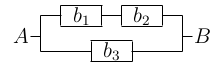
\includegraphics[width=.2\linewidth]{Assets/GudS-schaltung.png}\end{center}
    \begin{parts}
        \part Mit welcher Wahrscheinlichkeit ist der Stromfluss in gegebenen Schaltung von A nach B unterbrochen?
        \begin{solution}
        \end{solution}
        \part Um wieviele Bauteile der Sorte $b_3$ ist die in a) gezeigte Schaltung durch Parallelschaltung mindestens zu erweitern, damit die Ausfallwahrscheinlichkeit noch höchstens $0.0002$ beträgt?
        \begin{solution}
        \end{solution}
    \end{parts}

    \question Drei Personen besteigen in der Tiefgarage eines Gebäudes den Fahrstuhl und verlassen diesen unabhängig voneinander und jeweils mit gleicher Wahrscheinlichkeit in einem der folgenden 10 Etagen. Es bezeichne X die Anzahl der Fahrstuhlhalts, den die drei Fahrgäste benötigen. Berechnen Sie $P[X=k]$ für $1\leq k\leq 10$ und $E[X]$.
    \begin{solution}
    \end{solution}

    \question Zwei Unternehmen sind zu 60\% bzw. zu 40\% an der Gesamtproduktion eines elektronischen Bauteils beteiligt. Die Wahrscheinlichkeit, dass ein Bauteil mindestens 2000 Stunden betriebsfähig bleibt, ist für das erste Unternehmen $0.8$ und für das zweite Unternehmen $0.7$.
    \begin{parts}
        \part Mit welcher Wahrscheinlichkeit bleibt ein der Gesamtproduktion entnommenes Bauteil mindestens 2000 Stunden lang betriebsfähig?
        \begin{solution}
        \end{solution}
        \part Wie groß ist die Wahrscheinlichkeit dafür, dass ein beliebig ausgewähltes Bauteil, das bereits nach 1200 Stunden ausfiel, aus dem zweiten Unternehmen stammt?
        \begin{solution}
        \end{solution}
    \end{parts}

    \question In einer Spielshow stellt der Moderator den Kandidaten vor die Entscheidung, eines von drei Toren zu wählen. Hinter einem verbrirgt sich der Hauptpreis, hinter den zwei anderen der Zonk (eine Niete). Der Kandidat wählt eines der Tore. Daraufhin öffnet der Moderator eines der beiden anderen Tore hinter dem sich ein Zonk befindet und lässt dem Kandidaten die Wahl, das gewählte Tor zu behalten oder das verbleibende zu wählen. Sollte der Kandidat wechseln?
    \begin{solution}
    \end{solution}

    \question An der Technischen Universität Hintertupfingen studieren 10\% aller Studierenden Informatik, 15\% Angewandte Medienwissenschaften, 20\% beginnen ein Wirtschafts- und 55\% ein Ingenieurstudium. Im Wintersemester 2011/12 lag bei der Mathematik I Prüfung die Durchfallquote bei 50\% bei den Informatikern 35\% bei den Ingenieuren 30\% bei den Wirtschaftlern und bei den angewandten Medienwissenschaftlern bei 60\%. Im April läuft ein glücklich aussehender Student über den Campus, der gerade seine Mathe I Klausur bestanden hat. Wie groß ist die Wahrscheinlichkeit, dass er Informatiker ist?
    \begin{solution}
    \end{solution}

    \question Anna ist Informatikstudentin und besucht etwa jede 2. Woche ihre Lieblingsdiskothek. Diese hat 3 Räume, von denen Anna jeden gleich häufig besucht. Ihr Kommilitone Bastian besucht eines Samstags die Disko. Er trifft Anna in den ersten beiden Räumen nicht an. Wie groß ist die Wahrscheinlichkeit, dass Anna sich im dritten Raum befindet?
    \begin{solution}
    \end{solution}

    \question Bastian findet Anna nicht in der Disko, dafür aber zwei flüchtige Bekanntschaften namens Dorothea und Eleonore, die er gerne näher kennenlernen würde. Er schätzt die Chancen dazu bei Dorothea auf 70\% und bei Eleonore auf 50\%. Bei einem Misserfolg könnte er sein Glück noch bei der jeweils anderen versuchen. Dann hätte er nur noch eine 10\%ige Aussicht auf Erfolg, falls sein erster Versuch aufgefallen ist. Eleonore würde das sofort bemerken, Dorothea nur zu 50\%, da sie gerade etwas abgelenkt ist. In welcher Reihenfolge sollte Bastian die Damen ansprechen?
    \begin{solution}
    \end{solution}

    \question Ein Postbote soll ein Paket bei einem Empfänger abgeben. Trifft er diesen nicht an, wird der Postbote noch 3 weitere Zustellversuche machen ehe das Paket an den Absender zurückgeschickt wird. Die Ereignisse, den Empfänger an einem bestimmten Tag anzutreffen seien dabei unabhängig und haben die Wahrscheinlichkeit $p=0,3$.
    \begin{parts}
        \part Mit welcher Wahrscheinlichkeit erreicht das Paket den Empfänger?
        \begin{solution}
        \end{solution}
        \part Für die Zufallsgröße X der Anzahl der Zustellversuche gebe man Erwartungswert und Varianz an.
        \begin{solution}
        \end{solution}
    \end{parts}

    \question Ein Student mit Stochastik-Tick beschließt ein Jahr lang seine Samstagabendbeschäftigung dem Zufall zu überlassen. Er würfelt jeden Freitag einmal mit einem Würfel und entscheidet dann wie folgt: Er geht zum Tanz, falls die Augenzahl nicht größer als 4 ist, bei einer 5 liest er ein Buch und bei einer 6 geht er ins Kino. Nun sei das Jahr in 13 Perioden a 4 Wochen eingeteilt. Man bestimme die Wahrscheinlichkeit dafür, dass der Student in einer solchen Periode (z.B. der ersten):
    \begin{parts}
        \part mindestens einmal ein Buch liest,
        \begin{solution}
        \end{solution}
        \part 2 mal ins Kino geht,
        \begin{solution}
        \end{solution}
        \part 4 mal tanzen geht,
        \begin{solution}
        \end{solution}
        \part nie tanzen geht,
        \begin{solution}
        \end{solution}
        \part alle drei Beschäftigungen wenigstens einmal auftreten.
        \begin{solution}
        \end{solution}
        \part Außerdem bestimme man die zu erwartende Anzahl von Perioden, in denen er mindestens 3mal tanzen geht.
        \begin{solution}
        \end{solution}
    \end{parts}

    \question Beim Biathlon darf beim Schießen bei 5 Schüssen höchstens 2 mal nachgeladen werden, wenn nicht getroffen wurde. Ansonsten müssen Strafrunden gelaufen werden. Es bezeichne X die Anzahl der abgegebenen Schüsse und Y die Anzahl der Strafrunden. Berechnen Sie für beide Zufallsgrößen den Erwartungswert und die Varianz, wenn die Trefferwahrscheinlichkeit 80 Prozent beträgt.
    \begin{solution}
    \end{solution}

    \question 5 Personen fahren gemeinsam mit einem Auto von der Disko nach Hause. 2 von ihnen haben in der Diskothek Drogen konsumiert. Das Auto wird von der Polizei angehalten und zwei der Insassen werden zufällig zu einem Drogentest ausgewählt.
    \begin{parts}
        \part Für die Zufallsgröße X der positiv getesteten Personen bestimme man die Einzelwahrscheinlichkeiten sowie Erwartungswert und Varianz.
        \begin{solution}
        \end{solution}
        \part Der Test sei nun nicht ganz sicher sondern schlägt nur mit einer Wahrscheinlichkeit von 75\% an. (0\% falls keine genommen wurden). Y sei dann die Zufallsgröße der positiv getesteten Personen. Bestimmen Sie wieder Einzelwahrscheinlichkeiten, Erwartungswert und Varianz.
        \begin{solution}
        \end{solution}
        \part 100 der 1000 Besucher der Diskothek haben Drogen genommen. Die Polizei testet 20 Personen. Man bestimme näherungsweise die Wahrscheinlichkeit dafür, dass mindestens 3 von ihnen positiv getestet werden.
        \begin{solution}
        \end{solution}
    \end{parts}

    \question Es sei $G=(V,E)$ ein zusammenhängender Graph. Der graphentheoretische Abstand $d(x, y)$ der Ecken $x$ und $y$ ist die Länge eines kürzesten $x-y$-Weges. Man zeige, dass die Abbildung $d:V^2\rightarrow\mathbb{N}$ eine Metrik ist, d.h. für alle $x, y, z\in V$ gilt:
    \begin{itemize}
        \item $d(x,y)\geq 0$ und es gilt: $d(x,y)=0\Leftrightarrow x = y$ (positive Definitheit)
        \item $d(x,y) = d(y,x)$ (Symmetrie)
        \item $d(x,z)\leq d(x, y) + d(y,z)$ (Dreiecksungleichung)
    \end{itemize}
    \begin{solution}
    \end{solution}

    \question Es sei $G=(V,E)$ ein Graph. Man beweise, dass G genau dann nicht zusammenhängend ist, wenn es eine Partition $\{X,Y\}$ der Eckenmenge $V$ gibt, so dass keine Kante $xy\in E$ mit $x\in X$ und $y\in Y$ existiert.
    \begin{solution}
    \end{solution}

    \question Man beweise folgende Aussagen
    \begin{parts}
        \part In jedem Graphen ist die Anzahl der Ecken ungeraden Grades gerade.
        \begin{solution}
        \end{solution}
        \part Jeder Baum mit mindestens 2 Ecken hat eine Ecke vom Grad 1.
        \begin{solution}
        \end{solution}
        \part Jeder Baum T hat genau $|V(T)|-1$ Kanten.
        \begin{solution}
        \end{solution}
        \part Jeder Baum mit mindestens 2 Ecken hat mindesten 2 Ecken vom Grad 1.
        \begin{solution}
        \end{solution}
    \end{parts}

    \question Es sei $G=(V,E)$ ein zusammenhängender Graph. Man zeige, dass je zwei längste Wege eine Ecke gemeinsam haben.
    \begin{solution}
    \end{solution}

    \question Entscheiden Sie, ob es zu den angegebenen Knotengradfolgen einen Graphen gibt.
    \begin{parts}
        \part $1,2,3,3,4$
        \begin{solution}
        \end{solution}
        \part $1,2,2,2,3,6$
        \begin{solution}
        \end{solution}
        \part $2,2,3,3,4$
        \begin{solution}
        \end{solution}
    \end{parts}

    \question Beweisen Sie, dass in einem Graphen G, der verschieden vom Nullgraphen ist und dessen Knoten alle einen geraden Grad haben, die folgenden Aussagen gelten.
    \begin{itemize}
        \item G enthält einen Kreis.
        \item Es gibt eine Partition der Kantenmenge $E(G)$, deren Partitionsmengen gerade die Kantenmengen von Kreisen in $G$ sind.
    \end{itemize}
    \begin{solution}
    \end{solution}

    \question Zeigen Sie, dass jeder Graph mit $2n$ Ecken, der keinen Kreis der Länge 3 enthält, höchstens $n^2$ Kanten hat. (Hinweis: Induktion über n)
    \begin{solution}
    \end{solution}

\end{questions}
\end{document}